\documentclass[10pt]{beamer}
\usepackage[utf8x]{inputenc}
\usepackage[english]{babel}
\usetheme{Berlin}
\usepackage{thumbpdf}
\usepackage{wasysym}
\usepackage{ucs}
\beamertemplatenavigationsymbolsempty
%\usepackage {pgf,pgfarrows,pgfnodes,pgfautomata,pgfheaps,pgfshade}
\usepackage {verbatim}
\pdfinfo
{
  /Title       (Software Versioning )
  /Creator     (TeX)
  /Author      (Carlo Nicolini)
}

\title{Software versioning overview}
\subtitle{Subversion and Git at work}
\author{Carlo Nicolini}
\date{\today}

\begin {document}

%%%%%%%%%%%%%%%%%%%%%%%%%%%%%%%%%%%%%%%%%
%%%%%%%%%% INTRODUZIONE %%%%%%%%%%%%%%%%%
%%%%%%%%%%%%%%%%%%%%%%%%%%%%%%%%%%%%%%%%%

\section{Introduction}
\begin{frame}
\frametitle{Motivations}
Science nowadays is (mainly) about writing code.
\begin{block}{Programmer swiss-knife}
\begin{itemize}
\item<1-> A good book about the specific programming language (Matlab/Octave)
\item<2-> A good text editor (Notepad++ on Windows, TextMate on Mac, gedit on Ubuntu)
\item<3-> A good versioning system (Subversion or Git)
\item<4-> A way to keep backups
\end{itemize}
\end{block}
Everything else is accessory!
\end{frame}

%%%%%%%%%%%%%%%%%%%%%%%%%%%%%%%%%%%%%%%%%%%%%%%%%%%%%%%%%%%%%%%%%%%%%%%%%%%%%%%%%%%%%%%%%%%%
\begin{frame}
\frametitle{Why versioning?}
``Code doesn’t exist unless it’s checked into a version control system. Use version control for everything you do. Any version control, SVN, Git, even CVS, master it and use it.``

\begin{block}{Have you ever?}
\begin{small} 
\begin{itemize}
  \item  Made a change to code, realised it was a mistake and wanted to go back?
  \item  Lost code or had a backup that was too old?
  \item  Had to maintain multiple versions of a product?
  \item  Wanted to see the difference between two (or more) versions of your code?
  \item  Wanted to prove that a particular change broke or fixed some piece of code?
  \item  Wanted to see how much work is being done (where/when/who)?
  \item  Wanted to experiment with a new feature without interfering with working code?
 \end{itemize}
\end{small}
\end{block}
\end{frame}


%%%%%%%%%%%%%%%%%%%%%%%%%%%%%%%%%%%%%%%%%%%%%%%%%%%%%%%%%%%%%%%%%%%%%%%%%%%%%%%%%%%%%%%%%%%%
\begin{frame}
\frametitle{Even if you work alone}
You can always benefit from source control.
\begin{itemize}
 \item You don't lose anything.
 \item You can experiment at will.
\item You can revert!
\item You can look back in older versions where bug has been introduced/resolved.
\item You can see what changed.
\end{itemize}
\end{frame}



%%%%%%%%%%%%%%%%%%%%%%%%%%%%%%%%%%%%%%%%%%%%%%%%%%%%%%%%%%%%%%%%%%%%%%%%%%%%%%%%%%%%%%%%%%%%
\begin{frame}[fragile]
\frametitle{Is it for me?}
The response is YES if
\begin{itemize}
\item You mess around with multiple versions of files, multiple dates of same file.
\begin{itemize}
 \item  \begin{verbatim} experiment_6_december_NEW.m \end{verbatim}
 \item  \begin{verbatim} test_carlo_condition5_BACKUP.cpp \end{verbatim}
\end{itemize}

\item You have short memory
\item You have fun trying new disrupting features.
\item You like to collaborate with other persons.
\end{itemize}
\end{frame}


%%%%%%%%%%%%%%%%%%%%%%%%%%%%%%%%%%%%%%%%%%%%%%%%%%%%%%%%%%%%%%%%%%%%%%%%%%%%%%%%%%%%%%%%%%%%
\begin{frame}
\frametitle{What can I put under version control?}
Everything! Every file can be put under version control, but you get the most benefit from textual file.
\begin{block}{Files support}
\textbf{Best support} .cpp, .h, .c, .txt, .m, .tex, etc...

\textbf{Average support} Office files .doc, .docx, .pdf

\textbf{Bare copy, inefficient pick up} Binaries, pdfs, images, movies etc
\end{block}
\end{frame}
%%%%%%%%%%%%%%%%%%%%%%%%%%%%%%%%%%%%%%%%%%%%%%%%%%%%%%%%%%%%%%%%%%%%%%%%%%%%%%%%%%%%%%%%%%%%

%%%%%%%%%%%%%%%%%%%%%%%%%%%%%%%%%%%%%%%%%%%%%%%%%%%%%%%%%%%%%%%%%%%%%%%%%%%%%%%%%%%%%%%%%%%%
\begin{frame}[fragile]
 \frametitle{Subversion}
Subversion is one of the most used versioning systems.
\end{frame}

%%%%%%%%%%%%%%%%%%%%%%%%%%%%%%%%%%%%%%%%%%%%%%%%%%%%%%%%%%%%%%%%%%%%%%%%%%%%%%%%%%%%%%%%%%%%
\begin{frame}[fragile]
\frametitle{Centralized repository}
\begin{figure}[h]
 \centering
 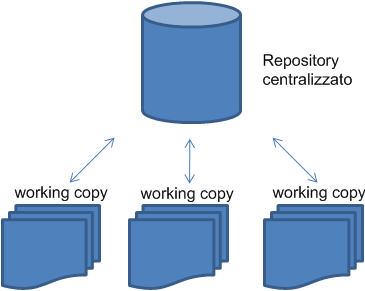
\includegraphics[width=0.5\textwidth]{images/svn-schema.png}
\end{figure}
Centralized repository in Subversion
\end{frame}
%%%%%%%%%%%%%%%%%%%%%%%%%%%%%%%%%%%%%%%%%%%%%%%%%%%%%%%%%%%%%%%%%%%%%%%%%%%%%%%%%%%%%%%%%%%%
\begin{frame}[fragile]
\frametitle{Subversion business logic - Working copy}
\begin{figure}[h]
 \centering
 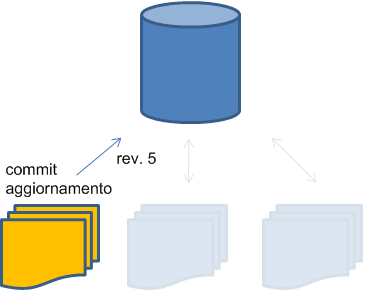
\includegraphics[width=0.5\textwidth]{images/svn-step2.png}
\end{figure}
User works on his own working copy and finally sends his modifications to remote repository.
\end{frame}

%%%%%%%%%%%%%%%%%%%%%%%%%%%%%%%%%%%%%%%%%%%%%%%%%%%%%%%%%%%%%%%%%%%%%%%%%%%%%%%%%%%%%%%%%%%%
\begin{frame}[fragile]
\frametitle{Subversion business logic - Working copy}
\begin{figure}[h]
 \centering
 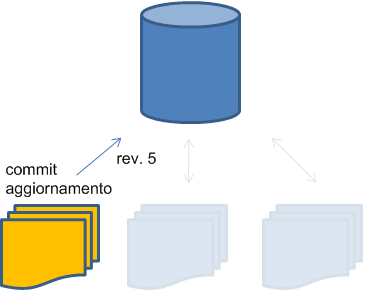
\includegraphics[width=0.5\textwidth]{images/svn-step2.png}
\end{figure}
User works on his own working copy and finally sends his modifications to remote repository.
\end{frame}

%%%%%%%%%%%%%%%%%%%%%%%%%%%%%%%%%%%%%%%%%%%%%%%%%%%%%%%%%%%%%%%%%%%%%%%%%%%%%%%%%%%%%%%%%%%%
\begin{frame}[fragile]
\frametitle{Subversion business logic - Edit}
\begin{figure}[h]
 \centering
 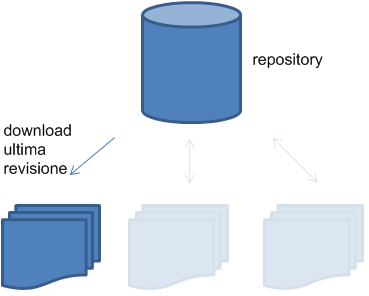
\includegraphics[width=0.5\textwidth]{images/svn-step1.png}
\end{figure}
A repository is like a data store.
Every user has a copy of the repository on his own computer (working copy)
\end{frame}

%%%%%%%%%%%%%%%%%%%%%%%%%%%%%%%%%%%%%%%%%%%%%%%%%%%%%%%%%%%%%%%%%%%%%%%%%%%%%%%%%%%%%%%%%%%%
\begin{frame}[fragile]
\frametitle{Subversion business logic - Sending local edits}
\begin{figure}[h]
 \centering
 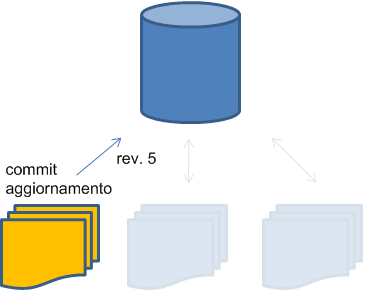
\includegraphics[width=0.5\textwidth]{images/svn-step2.png}
\end{figure}
The repository gets the ''commit'' from users, updates its internal status and increases the revision number.
\end{frame}


%%%%%%%%%%%%%%%%%%%%%%%%%%%%%%%%%%%%%%%%%%%%%%%%%%%%%%%%%%%%%%%%%%%%%%%%%%%%%%%%%%%%%%%%%%%%
\begin{frame}[fragile]
\frametitle{Subversion business logic - Handling conflicts}
\begin{figure}[h]
 \centering
 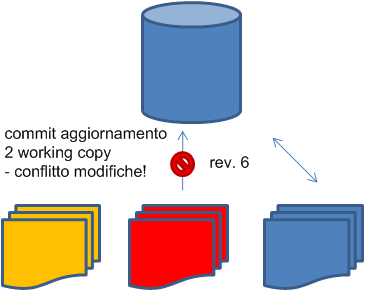
\includegraphics[width=0.5\textwidth]{images/svn-step3.png}
\end{figure}
A questo punto, chiunque può disporre della versione aggiornata. Nel caso in cui qualcuno tenti di inviare delle modifiche ad un file appena aggiornato, il repository inverà un messaggio d’avviso.
Attraverso i tool di SVN è possibile gestire quale revisione e quale singola modifica deve essere mantenuta.
In caso di conflitto, è possibile gestire il merge delle revisioni.
\end{frame}

%%%%%%%%%%%%%%%%%%%%%%%%%%%%%%%%%%%%%%%%%%%%%%%%%%%%%%%%%%%%%%%%%%%%%%%%%%%%%%%%%%%%%%%%%%%%
\begin{frame}[fragile]
\frametitle{Subversion business logic - Handling conflicts}
\begin{figure}[h]
 \centering
 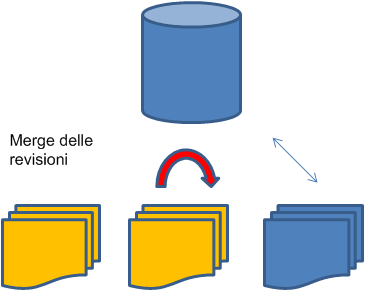
\includegraphics[width=0.5\textwidth]{images/svn-step4.png}
\end{figure}
A questo punto, chiunque può disporre della versione aggiornata. Nel caso in cui qualcuno tenti di inviare delle modifiche ad un file appena aggiornato, il repository inverà un messaggio d’avviso.
Attraverso i tool di SVN è possibile gestire quale revisione e quale singola modifica deve essere mantenuta.
In caso di conflitto, è possibile gestire il merge delle revisioni.
\end{frame}


%%%%%%%%%%%%%%%%%%%%%%%%%%%%%%%%%%%%%%%%%%%%%%%%%%%%%%%%%%%%%%%%%%%%%%%%%%%%%%%%%%%%%%%%%%%%
\begin{frame}[fragile]
\frametitle{Example usage}
\begin{figure}[h]
 \centering
 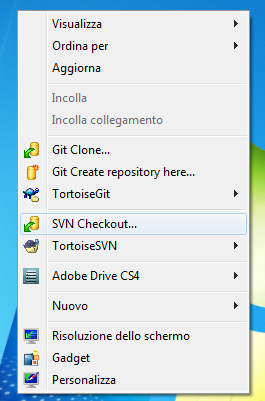
\includegraphics[width=0.35\textwidth]{images/image1.png}
\end{figure}
\begin{verbatim}
svn co svn+ssh://cncsuser@193.205.214.36/home/svn/testrepo 
\end{verbatim}
\end{frame}

%%%%%%%%%%%%%%%%%%%%%%%%%%%%%%%%%%%%%%%%%%%%%%%%%%%%%%%%%%%%%%%%%%%%%%%%%%%%%%%%%%%%%%%%%%%%
\begin{frame}[fragile]
\frametitle{Example usage}
\begin{figure}[h]
 \centering
 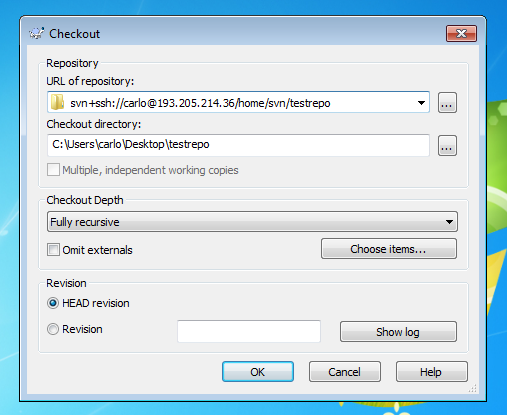
\includegraphics[width=0.6\textwidth]{images/image2.png}
\end{figure}
\begin{verbatim}
svn co svn+ssh://cncsuser@193.205.214.36/home/svn/testrepo 
\end{verbatim}
\end{frame}

%%%%%%%%%%%%%%%%%%%%%%%%%%%%%%%%%%%%%%%%%%%%%%%%%%%%%%%%%%%%%%%%%%%%%%%%%%%%%%%%%%%%%%%%%%%%
\begin{frame}[fragile]
\frametitle{Example usage}
\begin{figure}[h]
 \centering
 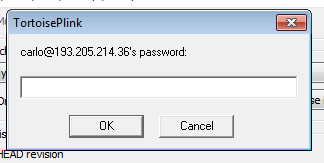
\includegraphics[width=0.6\textwidth]{images/image3.png}
\end{figure}
Insert your password here
\end{frame}

%%%%%%%%%%%%%%%%%%%%%%%%%%%%%%%%%%%%%%%%%%%%%%%%%%%%%%%%%%%%%%%%%%%%%%%%%%%%%%%%%%%%%%%%%%%%
\begin{frame}[fragile]
\frametitle{Example usage}
\begin{figure}[h]
 \centering
 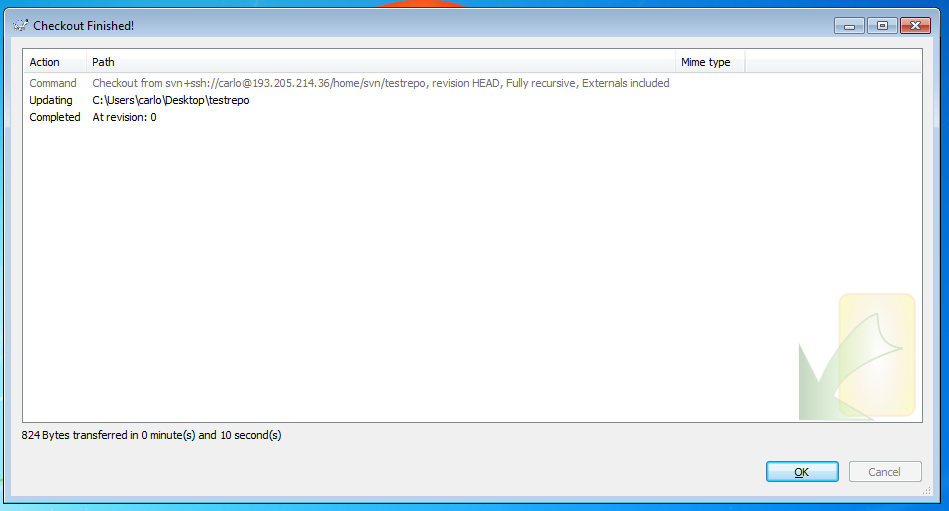
\includegraphics[width=1.0\textwidth]{images/image4.png}
\end{figure}
Here is the checkout log
\end{frame}

%%%%%%%%%%%%%%%%%%%%%%%%%%%%%%%%%%%%%%%%%%%%%%%%%%%%%%%%%%%%%%%%%%%%%%%%%%%%%%%%%%%%%%%%%%%%
\begin{frame}[fragile]
\frametitle{Example usage}
\begin{figure}[h]
 \centering
 
\includegraphics[width=0.5\textwidth]{images/image5.png}
\end{figure}
Green icon means that the repository has NO local modifications and is in sync with the last update.
\end{frame}

%%%%%%%%%%%%%%%%%%%%%%%%%%%%%%%%%%%%%%%%%%%%%%%%%%%%%%%%%%%%%%%%%%%%%%%%%%%%%%%%%%%%%%%%%%%%
\begin{frame}[fragile]
\frametitle{Example usage}
\begin{figure}[h]
 \centering
 
\includegraphics[width=0.7\textwidth]{images/image6.png}
\end{figure}
Adding a new file, this will NOT be under version control!
\begin{verbatim}
 touch MyTextFile.txt
\end{verbatim}
\end{frame}

%%%%%%%%%%%%%%%%%%%%%%%%%%%%%%%%%%%%%%%%%%%%%%%%%%%%%%%%%%%%%%%%%%%%%%%%%%%%%%%%%%%%%%%%%%%%
\begin{frame}[fragile]
\frametitle{Example usage}
\begin{figure}[h]
 \centering
 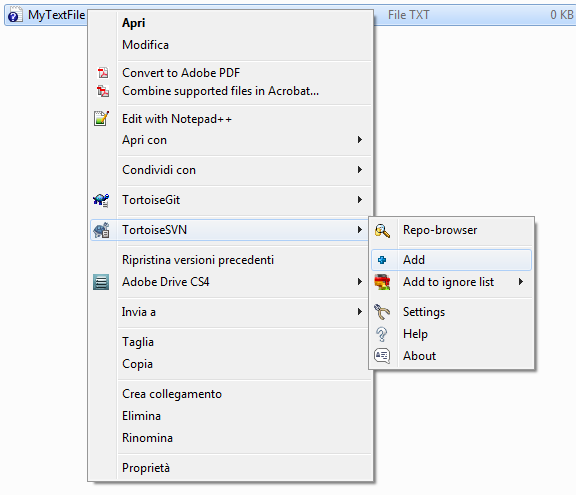
\includegraphics[width=0.7\textwidth]{images/image7.png}
\end{figure}
Adding a new file, now it WILL be under version control
\begin{verbatim}
svn add MyTextFile.txt
\end{verbatim}
\end{frame}

%%%%%%%%%%%%%%%%%%%%%%%%%%%%%%%%%%%%%%%%%%%%%%%%%%%%%%%%%%%%%%%%%%%%%%%%%%%%%%%%%%%%%%%%%%%%
\begin{frame}[fragile]
\frametitle{Example usage}
\begin{figure}[h]
 \centering
 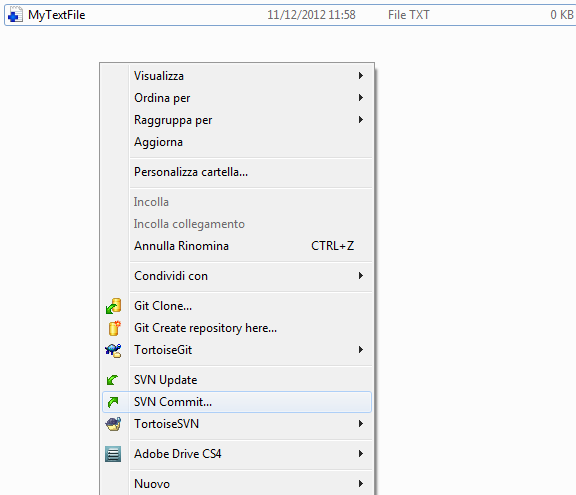
\includegraphics[width=0.7\textwidth]{images/image8.png}
\end{figure}
Commit the file addition, so the remote repository will be informed of our new file creation.
\begin{verbatim}
svn commit -m "added a new file MyTextFile.txt to the repository"
\end{verbatim}
\end{frame}

%%%%%%%%%%%%%%%%%%%%%%%%%%%%%%%%%%%%%%%%%%%%%%%%%%%%%%%%%%%%%%%%%%%%%%%%%%%%%%%%%%%%%%%%%%%%
\begin{frame}[fragile]
\frametitle{Example usage}
\begin{figure}[h]
 \centering
 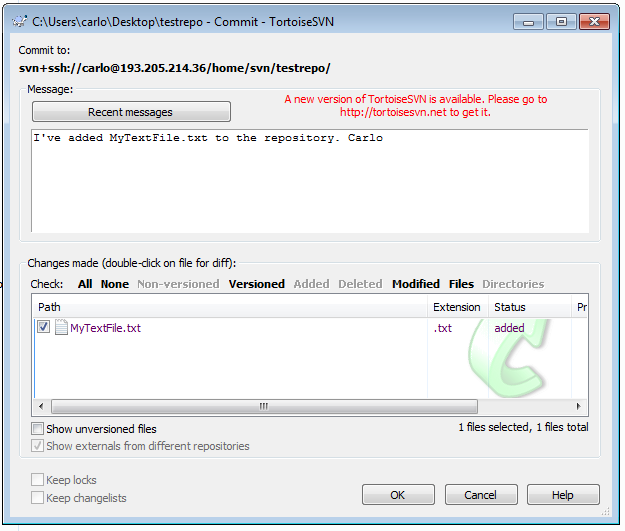
\includegraphics[width=0.7\textwidth]{images/image9.png}
\end{figure}
\begin{verbatim}
svn commit -m "added a new file MyTextFile.txt"
\end{verbatim}
\end{frame}

%%%%%%%%%%%%%%%%%%%%%%%%%%%%%%%%%%%%%%%%%%%%%%%%%%%%%%%%%%%%%%%%%%%%%%%%%%%%%%%%%%%%%%%%%%%%
\begin{frame}[fragile]
\frametitle{Example usage}
\begin{figure}[h]
 \centering
 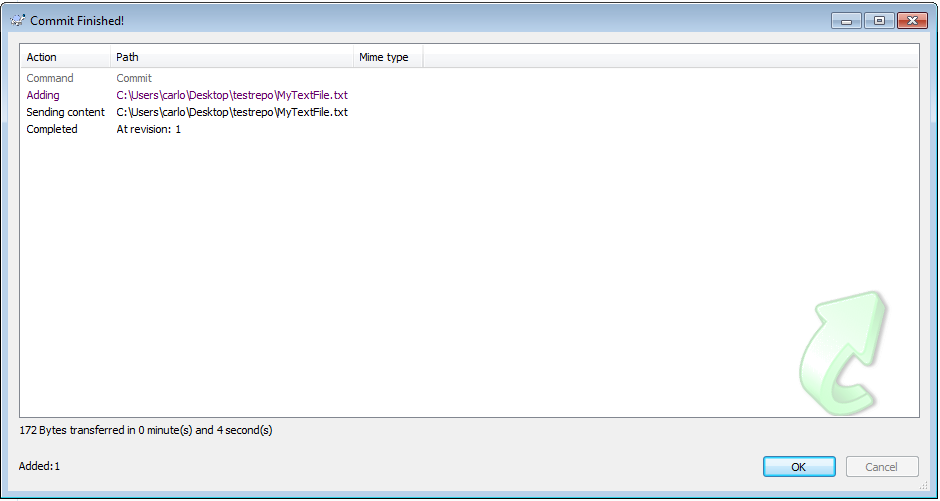
\includegraphics[width=1.0\textwidth]{images/image10.png}
\end{figure}
SVN log while committing to remote repository. You must see NO errors or red texts!
\end{frame}


%%%%%%%%%%%%%%%%%%%%%%%%%%%%%%%%%%%%%%%%%%%%%%%%%%%%%%%%%%%%%%%%%%%%%%%%%%%%%%%%%%%%%%%%%%%%
\begin{frame}[fragile]
\frametitle{Example usage}
\begin{figure}[h]
 \centering
 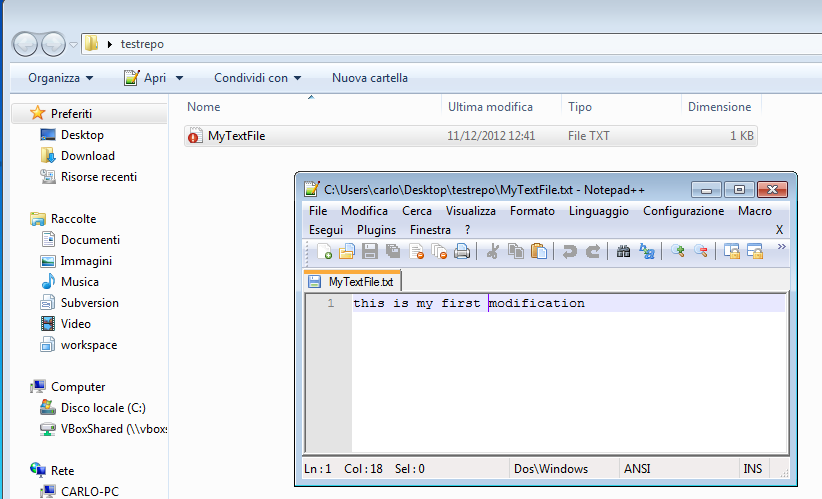
\includegraphics[width=1.0\textwidth]{images/image11.png}
\end{figure}
Doing modification on our file, will make the green icon red, because is locally modified
\end{frame}

%%%%%%%%%%%%%%%%%%%%%%%%%%%%%%%%%%%%%%%%%%%%%%%%%%%%%%%%%%%%%%%%%%%%%%%%%%%%%%%%%%%%%%%%%%%%
\begin{frame}[fragile]
\frametitle{Example usage}
\begin{figure}[h]
 \centering
 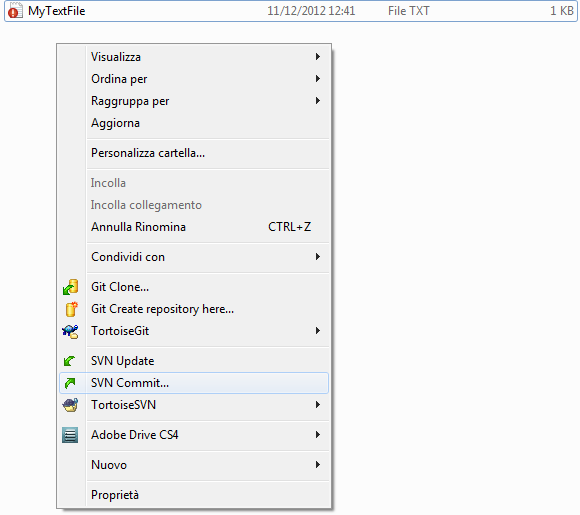
\includegraphics[width=0.7\textwidth]{images/image12.png}
\end{figure}
Commit again to push the local modifications to the remote repository
\end{frame}

%%%%%%%%%%%%%%%%%%%%%%%%%%%%%%%%%%%%%%%%%%%%%%%%%%%%%%%%%%%%%%%%%%%%%%%%%%%%%%%%%%%%%%%%%%%%
\begin{frame}[fragile]
\frametitle{Example usage}
\begin{figure}[h]
 \centering
 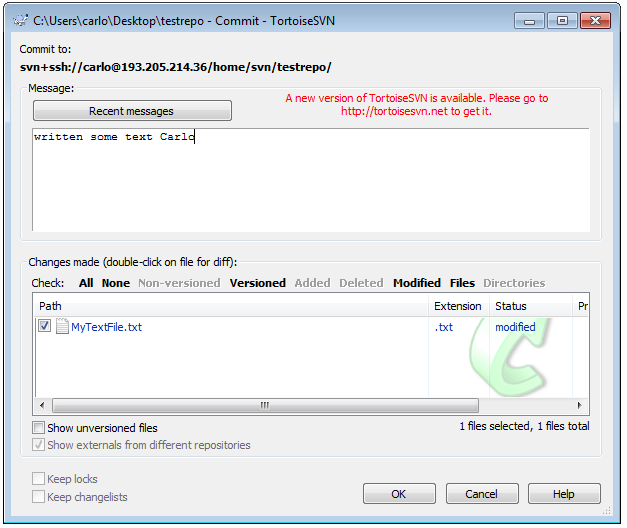
\includegraphics[width=0.7\textwidth]{images/image13.png}
\end{figure}
\begin{verbatim}
 svn commit -m "written some text."
\end{verbatim}
\end{frame}

%%%%%%%%%%%%%%%%%%%%%%%%%%%%%%%%%%%%%%%%%%%%%%%%%%%%%%%%%%%%%%%%%%%%%%%%%%%%%%%%%%%%%%%%%%%%
\begin{frame}[fragile]
\frametitle{Keeping track of history}
\begin{figure}[h]
 \centering
 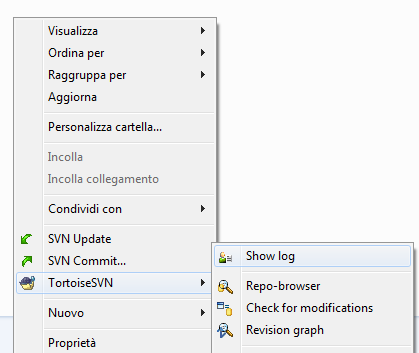
\includegraphics[width=0.7\textwidth]{images/image14.png}
\end{figure}
\begin{verbatim}
 svn log | head -100
\end{verbatim}
\end{frame}

%%%%%%%%%%%%%%%%%%%%%%%%%%%%%%%%%%%%%%%%%%%%%%%%%%%%%%%%%%%%%%%%%%%%%%%%%%%%%%%%%%%%%%%%%%%%
\begin{frame}[fragile]
\frametitle{Keeping track of history}
\begin{figure}[h]
 \centering
 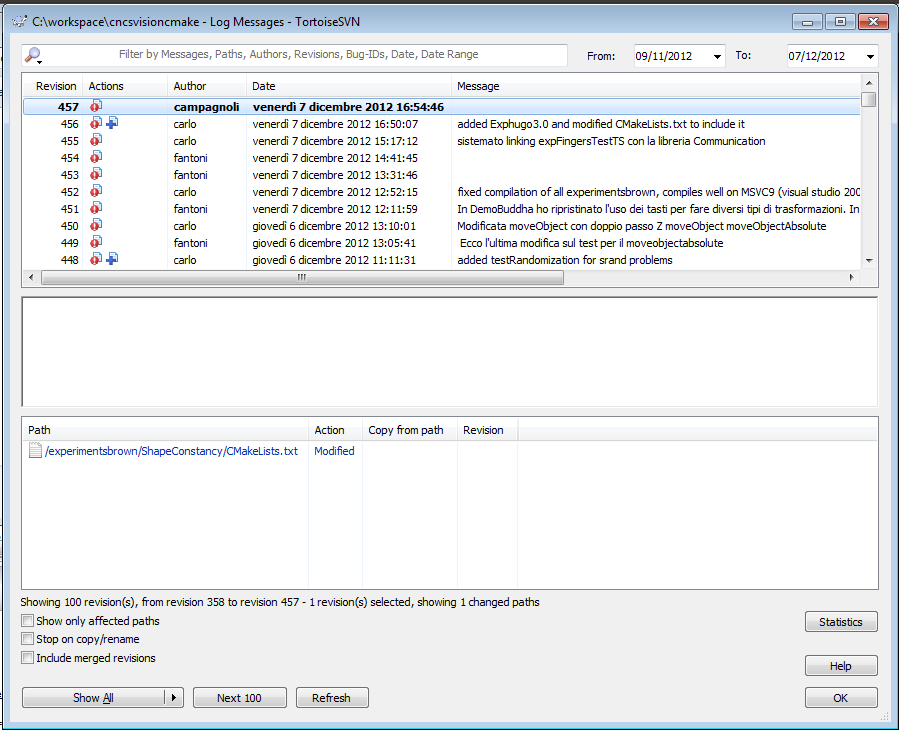
\includegraphics[width=0.7\textwidth]{images/image15.png}
\end{figure}
\begin{verbatim}
 svn log | head -100
\end{verbatim}
\end{frame}

%%%%%%%%%%%%%%%%%%%%%%%%%%%%%%%%%%%%%%%%%%%%%%%%%%%%%%%%%%%%%%%%%%%%%%%%%%%%%%%%%%%%%%%%%%%%
\begin{frame}[fragile]
\frametitle{How to avoid getting prompted for password (TortoiseSVN)}
\begin{figure}[h]
 \centering
 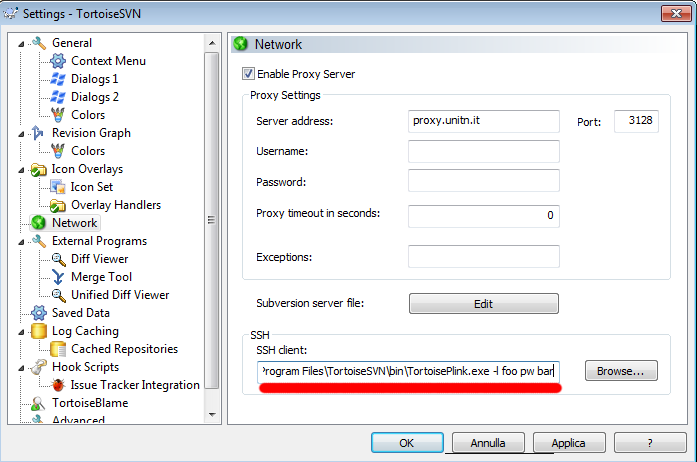
\includegraphics[width=0.7\textwidth]{images/image16.png}
\end{figure}
WARNING: password is visible to everyone
\end{frame}

\end{document}
